\documentclass[tikz]{standalone}

\usetikzlibrary{shapes,arrows,shadows,calc, angles}
\usetikzlibrary{arrows,shapes}
\usetikzlibrary{positioning}
\usetikzlibrary{patterns.meta}
\usetikzlibrary{decorations, decorations.pathreplacing}

\definecolor{fg}{rgb}{0,0,0}
\definecolor{bg}{rgb}{1,1,1}

\tikzstyle{box}=[draw, rounded corners , text width=40mm,
anchor=center,text centered,text=fg, font=\bfseries] % text width=33mm,

\tikzstyle{myarrow}=[->, >=stealth, very thick, rounded corners=2mm]
\tikzstyle{mythinarrow}=[myarrow, line width=0.25mm]

\tikzstyle{residuel}=[box, fill=red!60]
\tikzstyle{dconv}=[box, fill=green!60]
\tikzstyle{concatenation}=[box, fill=cyan!60]

\begin{document}

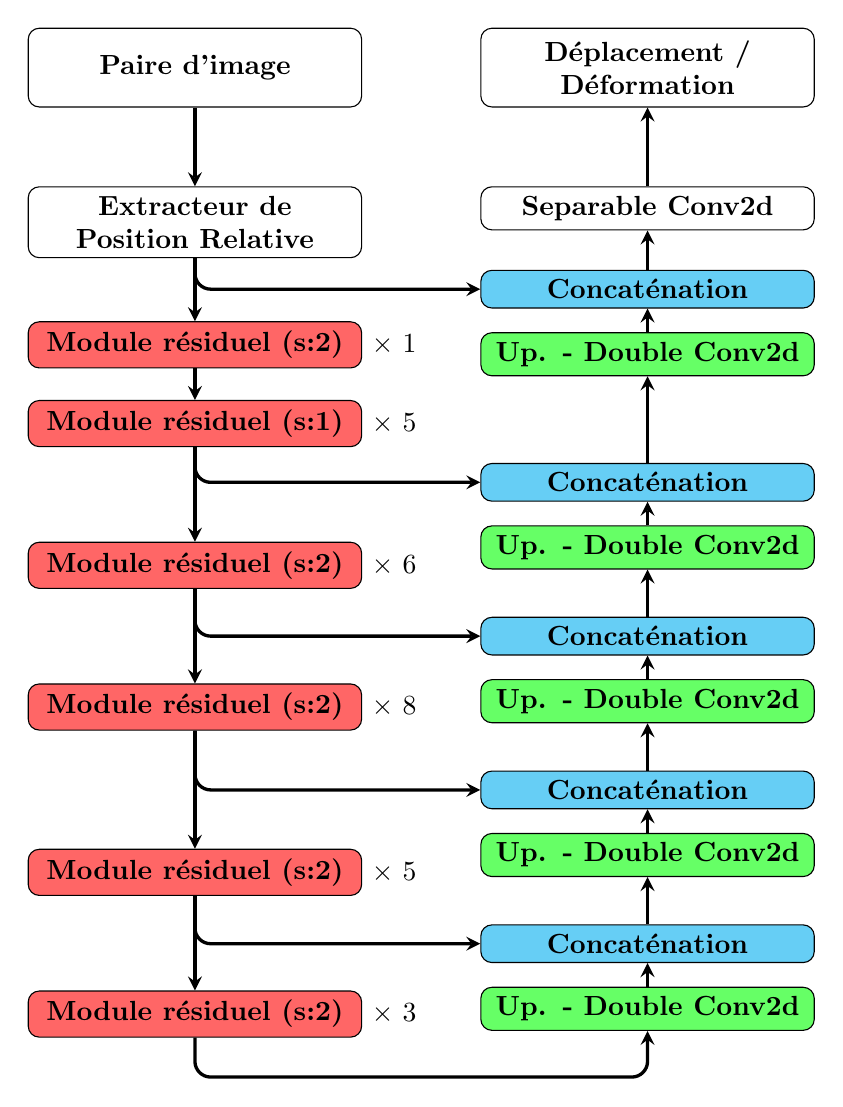
\begin{tikzpicture}

    \node[box,minimum height=10mm] (X) {Paire d'image};
    
    \node[box, right= of X, xshift=5mm, minimum height=10mm,] (Y) {Déplacement / Déformation} ;
    \node[box, below= of Y] (convLast) {Separable Conv2d } ;
    \draw[myarrow] (convLast) -- (Y) ;
    
    % CONCAT 0
    \node[concatenation, below= of convLast, yshift=5mm] (concat0) {Concaténation} ;
    \draw[myarrow] (concat0) -- (convLast) ;

    \node[box, below=of X] (RPE) {Extracteur de Position Relative} ;
    \draw[myarrow] (X) -- (RPE) ;
    \draw[myarrow] (RPE) |- (concat0) ;

    % DOUBLE CONV 0
    \node[dconv, below= of concat0, yshift=7mm] (dblConv0) {Up. - Double Conv2d} ;
    \draw[myarrow] (dblConv0) -- (concat0) ;

    % CONCAT 1
    \node[concatenation, below= of dblConv0, yshift=-1mm] (concat1) {Concaténation} ;
    \draw[myarrow] (concat1) -- (dblConv0) ;

    % DOUBLE CONV 1
    \node[dconv, below= of concat1, yshift=7mm] (dblConv1) {Up. - Double Conv2d} ;
    \draw[myarrow] (dblConv1) -- (concat1) ;

    % CONCAT 2
    \node[concatenation, below= of dblConv1, yshift=4mm] (concat2) {Concaténation} ;
    \draw[myarrow] (concat2) -- (dblConv1) ;


    % DOUBLE CONV 2
    \node[dconv, below= of concat2, yshift=7mm] (dblConv2) {Up. - Double Conv2d} ;
    \draw[myarrow] (dblConv2) -- (concat2) ;

    % CONCAT 3
    \node[concatenation, below= of dblConv2, yshift=4mm] (concat3) {Concaténation} ;
    \draw[myarrow] (concat3) -- (dblConv2) ;

    % DOUBLE CONV 3
    \node[dconv, below= of concat3, yshift=7mm] (dblConv3) {Up. - Double Conv2d} ;
    \draw[myarrow] (dblConv3) -- (concat3) ;

    % CONCAT 4
    \node[concatenation, below= of dblConv3, yshift=4mm] (concat4) {Concaténation} ;
    \draw[myarrow] (concat4) -- (dblConv3) ;

    % DOUBLE CONV 4
    \node[dconv, below= of concat4, yshift=7mm] (dblConv4) {Up. - Double Conv2d} ;
    \draw[myarrow] (dblConv4) -- (concat4) ;

    % RES 1
    \node[residuel, below=of RPE, yshift=2mm] (Res1) {Module résiduel (s:2)} ;
    \draw[myarrow] (RPE) -- (Res1) ;
    \node[right=of Res1, xshift=-10mm] {$\times$~1} ;

    % RES 2
    \node[residuel, below=of Res1, yshift=6mm] (Res2) {Module résiduel (s:1)} ;
    \draw[myarrow] (Res1) -- (Res2) ;
    \draw[myarrow] (Res2) |- (concat1) ;
    \node[right=of Res2, xshift=-10mm] {$\times$~5} ;

    % RES 3
    \node[residuel, below=of Res2, yshift=-2mm] (Res3) {Module résiduel (s:2)} ;
    \draw[myarrow] (Res2) -- (Res3) ;
    \draw[myarrow] (Res3) |- (concat2) ;
    \node[right=of Res3, xshift=-10mm] {$\times$~6} ;
    
    % RES 4
    \node[residuel, below=of Res3, yshift=-2mm] (Res4) {Module résiduel (s:2)} ;
    \draw[myarrow] (Res3) -- (Res4) ;
    \draw[myarrow] (Res4) |- (concat3) ;
    \node[right=of Res4, xshift=-10mm] {$\times$~8} ;
    
    \node[residuel, below=of Res4, yshift=-5mm] (Res5) {Module résiduel (s:2)} ;
    \draw[myarrow] (Res4) -- (Res5) ;
    \draw[myarrow] (Res5) |- (concat4) ;
    \node[right=of Res5, xshift=-10mm] {$\times$~5} ;

    \node[residuel, below=of Res5, yshift=-2mm] (Res6) {Module résiduel (s:2)} ;
    \draw[myarrow] (Res5) -- (Res6) ;
    \draw[myarrow] (Res6) -- ++ (0, -8mm) -| (dblConv4) ;
    \node[right=of Res6, xshift=-10mm] {$\times$~3} ;

\end{tikzpicture}

\end{document}